\section{Theorie} 
\label{sec:theorie}

\subsection{Ablenkung von Elektronen im elektrischen Feld}
\label{sec:ablenkung_efeld}

    Im Folgenden sollen die theoretischen Grundlagen der Ablenkung von Elektronen in einem elektrischen Feld erläutert werden.

\subsubsection{Die Kathodenstrahlröhre}
\label{sec:kathodenstrahlröhre}

    Für die Untersuchung der Ablenkung von Elektronen wird eine Kathodenstrahlröhre verwendet,
    welche auf einen Druck von $\SI{e-6}{\milli\bar}$ evakuiert ist,
    um Wechselwirkungen zwischen Elektronen und Luftmolekülen zu minimieren.\\
    Der Aufbau der Kathodenstrahlröhre ist in der folgenden Abbildung gezeigt.
    \begin{figure}[H]
        \centering
        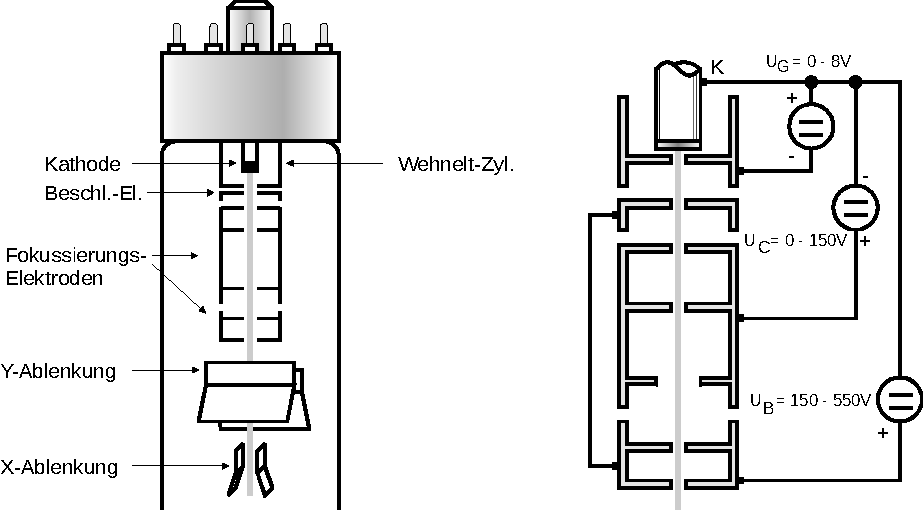
\includegraphics[scale=0.9]{content/img/V501/Abb_1.pdf}
        \caption{Der Aufbau einer Kathodenstrahlröhre.}
        \label{fig:kathodenstrahlröhre_querschnitt}
    \end{figure}
    Die Kathodenstrahlröhre setzt sich aus drei Hauptbestandteilen zusammen,
    einer Elektronenkanone und einem Ablenk-/ und Nachweissystem.\\
    Die Elektronen werden von der Elektronenkanone erzeugt und beschleunigt.
    Diese besteht aus einer negativ geladenen, zylinderförmigen Kathode,
    welche eine geringe Austrittsarbeit besitzt,
    sodass beim Heizen der Kathode mit einer Heizspannung $U_\text{G}$ Elektronen aus der Kathode austreten können.
    Die Elektronen werden mithilfe einer Beschleunigungsspannung $U_\text{B}$ zu einer positiv geladenen Elektrode hin beschleunigt,
    wobei die Intensität des Elektronenstrahls durch einen gleich negativ geladenen Wehnelt-Zylinder,
    welcher um die Kathode herum angebracht ist,
    kontrolliert wird.
    Nach der Energieerhaltung $E_\text{Kin} = E_\text{El}$ gilt bei der Beschleunigung der Elektronen
    \begin{equation}
        \frac{m_0 v^2_\text{z}}{2} = e_0 U_\text{B}
        \label{eqn:energieerhaltung_beschleunigung}
    \end{equation} 
    mit der Elektronenmasse $m_0$ und ihrer Ladung $e_0$.
    Der Faktor $v_\text{z}$ stellt die Geschwindigkeit der Elektronen dar, 
    welche sich in z-Richtung bewegen.
    Anschließend wird der Elektronenstrahl mithilfe mehrere elektrischer Linsen auf einen Leuchtschirm fokussiert.
    Die Linsen setzen sich aus Elektroden zusammen,
    zwischen denen inhomogene,
    elektrische Felder herrschen,
    welche mit einer Spannung $U_\text{C}$ eingestellt werden können.\\
    \\
    Nachdem der Elektronenstrahl fokussiert wurde,
    gelangt er in das Ablenksystem der Kathodenstrahlröhre,
    welches aus zwei Platten besteht,
    die parallel zueinander sind und an die eine Spannung $U_\text{d}$ angelegt ist,
    wodurch zwischen den Platten ein homogenes elektrisches Feld entsteht,
    für das näherungsweise
    \begin{equation*}
        E = \frac{U_\text{d}}{d}
    \end{equation*}
    gilt.
    Der Abstand $d$ der Platten muss dabei klein gegenüber ihrer Länge $p$ sein,
    sodass das Feld außerhalb verschwindet.
    \begin{figure}[H]
       \centering
        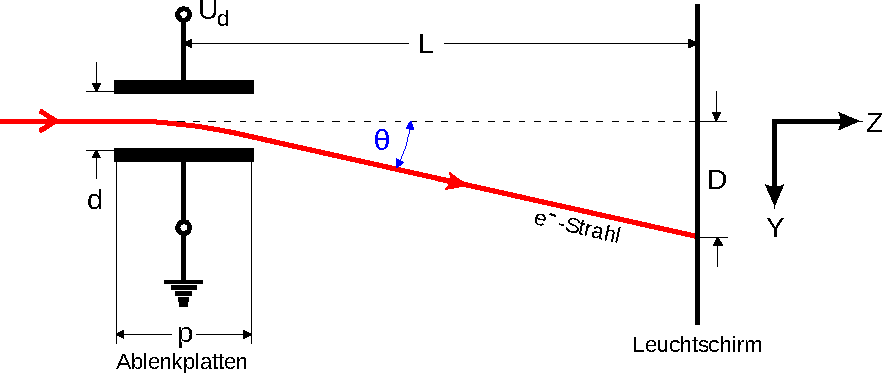
\includegraphics[scale=1]{content/img/V501/Abb_2.pdf}
        \caption{Ablenksystem der Kathodenstrahlröhre.}
        \label{fig:ablenkung}
    \end{figure}
    Die Abbildung \ref{fig:ablenkung} zeigt den Aufbau der Platten,
    welche sich im Abstand $L$ zum Schirm befinden.\\
    Im elektrischen Feld zwischen den Platten wirkt die konstante Kraft 
    \begin{equation*}
        \lvert \vec{F} \rvert = e_0 \frac{U_\text{d}}{d}
    \end{equation*}
    auf die Elektronen,
    sodass sie gleichmäßig während der Zeit $\symup{\Delta}t$,
    in der sich die Elektronen im elektrischen Feld befinden,
    gleichmäßig beschleunigt in y-Richtung abgelenkt werden.
    Die Geschwindigkeit des Elektronenstrahls nach Verlassen des Feldes zwischen den Platten wird mithilfe von 
    \begin{equation} 
        v_\text{y} = \frac{e_0}{m_0} \frac{U_\text{d}}{d} \frac{p}{v_\text{z}}
    \end{equation}
    beschrieben, 
    wobei $\symup{\Delta}t = p/v_\text{z}$ gilt,
    mit der ursprünglischen Geschwindigkeit $v_\text{z}$ der Elektronen in z-Richtung.
    %Nachdem die Elektronen das elektrische Feld verlassen haben,
    %bewegen sie sich wieder gleichförmig.
    \\
    Der Elektronenstrahl wird um den Winkel $\theta$ abgelenkt,
    welcher,
    unter Berücksichtigung der Kleinwinkelnäherung, 
    mit 
    \begin{align}
        \theta &\cong \frac{v_\text{y}}{v_\text{z}} 
        \intertext{oder dementsprechend}
        \theta &= \frac{e_0}{m_0} \frac{U_\text{d}}{d} \frac{p}{v^2_\text{z}}
    \end{align}
    berechnet werden kann.\\
    Aufgrund der Ablenkung wird der Punkt,
    auf dem die Elektronen auf den Leuchtschirm auftreffen,
    verschoben.
    Die Verschiebung $D$ kann durch
    \begin{equation}
        D = \theta L = \frac{p}{2d} L \frac{U_\text{d}}{U_\text{B}}
        \label{eqn:verschiebung}
    \end{equation}
    unter Verwendung der Gleichung \ref{eqn:energieerhaltung_beschleunigung} bestimmt werden.\\
    Da die Verschiebung $D$ proportional zur Ablenkspannung $U_\text{d}$ ist,
    kann mithilfe der Kathodenstrahlröhre eine Spannung gemessen werden.\\
    \\
    Wenn die Elektronen auf den Leuchtschirm treffen,
    regen sie Aktivatorzentren,
    Störstellen im Kristallgitter des Materials,
    an,
    welche Photonen emittieren,
    sodass der Auftreffpunkt sichtbar wird.
    Dies ist das Nachweissystem der Kathodenstrahlröhre.\\
    \\
    Für eine hohe Ablenkempfindlichkeit wird nach der Gleichung \ref{eqn:verschiebung} ein großer Abstand $L$,
    auch Strahlweg genannt,
    zwischen den Ablenkplatten und dem Leuchtschirm benötigt,
    sowie eine kleine Beschleunigungsspannung $U_\text{B}$ und eine große Plattenlänge $p$.\\
    Mit der Kathodenstrahlröhre können nur niederfrequente Wechselspannungen gemessen werden,
    da die Aufenthaltsdauer $\symup{\Delta}t$ klein gegenüber der Periodendauer von $U_\text{d}$ sein muss.
    Für eine \enquote{schnelle} Röhre werden eine geringe Plattenlänge $p$ und eine hohe Beschleunigungsspannung $U_\text{B}$ benötigt.

\subsubsection{Der Kathodenstrahl-Oszillograph} 
\label{sec:oszillograph}

    Um die Zeitabhängigkeiten von Wechselspannungen darzustellen,
    wird der Elektronenstrahl,
    wie in Abbildung \ref{fig:kathodenstrahlröhre_querschnitt} gezeigt,
    nach der Ablenkung in y-Richtung auch in x-Richtung abgelenkt.\\
    Dazu wird an das entsprechende Plattenpaar eine Sägezahnspannung angelegt,
    also eine Spannung,
    die periodisch linear anwächst und nach Erreichen eines Maximums sofort auf den Ursprungswert zurückspringt.
    Für die Frequenzen der Wechsel- und Sägezahnspannung ist die folgende Bedingung gegeben
    \begin{equation}
        n \cdot \nu_\text{Sä} = m \cdot \nu_\text{We} 
        \label{eqn:synchronisationsbedingung}
    \end{equation}
    mit $n,m \in \symbb{N}$,
    sodass der Verlauf der Wechselspannung sichtbar gemacht werden kann.

\subsection{Ablenkung von Elektronen im transversalen Magnetfeld}
\label{sec:ablenkung_bfeld}

    Im Folgenden sollen die theoretischen Grundlagen der Ablenkung von Elektronen in einem transversalen Magnetfeld erläutert werden.

\subsubsection{Die Bahn der Elektronen im Magnetfeld}

    In einem Magnetfeld wird nur auf bewegte Ladungen eine Kraft ausgeübt.
    Diese wird Lorentzkraft genannt und kann durch 
    \begin{equation*}
        \vec{F_\text{L}} = q \vec{v} \times \vec{B}
    \end{equation*}
    beschrieben werden, 
    wobei $q$ die Ladung eines Teilchens darstellt,
    das sich mit der Geschwindigkeit $\vec{v}$ senkrecht zum homogenen Magnetfeld $\vec{B}$ fortbewegt.\\
    Für ein Elektron mit der Ladung $e_0$,
    das sich mit einer konstanten Geschwindigkeit $v_0$ in z-Richtung durch ein homogenes Magnetfeld $B$,
    welches in x-Richtung wirkt,
    bewegt,
    ergibt sich demnach eine Kraft
    \begin{equation*}
        F_{L_y} = e_0 v_0 B
    \end{equation*}
    in y-Richtung.
    Die Kraft sorgt dafür,
    dass die Bahn des Elektrons in yz-Richtung gekrümmt wird.
    Da die Lorentzkraft immer senkrecht zur Bewegungsrichtung wirkt,
    ist die potentielle,
    und damit auch die kinetische Energie der Elektronen konstant,
    woraus folgt,
    dass in allen Punkten für die Geschwindigkeit
    \begin{equation*}
        \lvert \vec{v} \rvert = v_0 
    \end{equation*}
    gilt.\\
    Aufgrund des Gleichgewichts zwischen Lorentzkraft und Zentripetalkraft bei der Ablenkung der Elektronen ergibt sich für den Bahnradius
    \begin{equation}
        r = \frac{m_0 v_0}{e_0 B}
        \label{eqn:bahnradius}
    \end{equation}
    mit der Elektronenmasse $m_0$.
    Die Elektronen bewegen sich auf einer Kreisbahn.\\
    \\
    \\
    Mithilfe der Ablenkung der Elektronen im Magnetfeld und einer Kathodenstrahlröhre aus Kapitel \ref{sec:ablenkung_efeld} kann die spezifische Ladung $e_0/m_0$ der Elektronen bestimmt werden.\\
    \\
    Nachdem die Elektronen in der Kathodenstrahlröhre durch die Beschleunigungsspannung $U_\text{B}$ beschleunigt wurden,
    haben sie nach Gleichung \ref{eqn:energieerhaltung_beschleunigung} die konstante Geschwindigkeit
    \begin{equation}
        v_0 = \sqrt{2 U_\text{B} \frac{e_0}{m_0}} \ ,
    \end{equation}
    wobei hier $v_0 = v_\text{z}$ ist.
    Die folgende Abbildung zeigt die Bahn der Elektronen nach Eintreten in ein Magnetfeld.
    \begin{figure}[H]
       \centering
        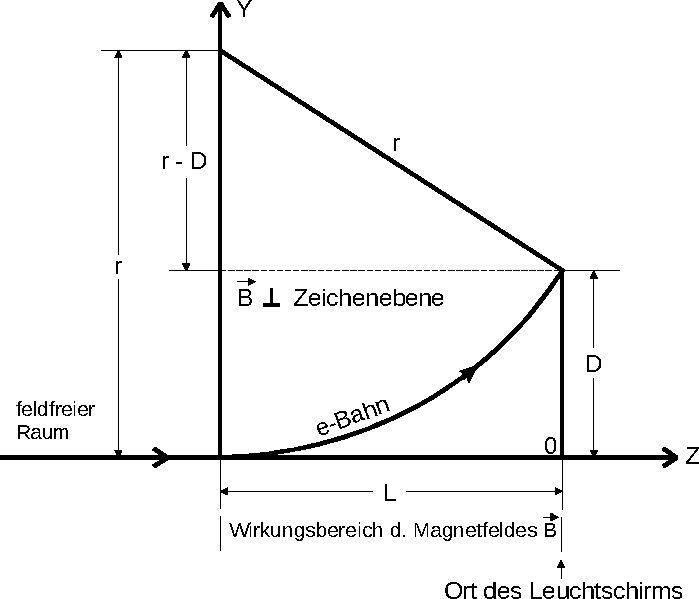
\includegraphics[scale=0.9]{content/img/V502/Abb_1.pdf}
        \caption{Bahn der Elektronen in einem Magnetfeld und dadurch erzeugte Verschiebung $D$ des Leuchtflecks auf dem Schirm.}
        \label{fig:elektronenbahn_magnetfeld}
    \end{figure}
    Solange sich die Elektronen noch nicht im magnetischen Feld befinden,
    bewegen sie sich geradlinig.
    Im Magnetfeld werden sie auf eine Bahn gelenkt,
    sodass sich der Punkt,
    an dem sie auf den Leuchtschirm in der Kathodenstrahlröhre treffen,
    verschiebt.
    Für den Bahnradius ergibt sich mit der Verschiebung $D$ und der Länge $L$ des Magnetfelds
    \begin{equation}
        r = \frac{L^2 + D^2}{2D} \ .
    \end{equation}
    Dieser Ausdruck kann mit Gleichung \ref{eqn:bahnradius} gleichgesetzt werden,
    sodass sich die messbare Größe
    \begin{equation}
        \frac{D}{L^2 + D^2} = \frac{1}{\sqrt{8 U_\text{B}}} \sqrt{\frac{e_0}{m_0}} B
        \label{eqn:formel_verschiebung}
    \end{equation}
    ergibt,
    mit der sich die spezifische Ladung der Elektronen berechnen lässt.